\chapter{Applicazione desktop}
\label{Cha:desktop}
\thispagestyle{empty}

Il capitolo seguente sarà incentrato sulla presentazione dell'applicazione desktop e delle sue interfacce e funzionalità.


\section{Sviluppo applicazione desktop}

L'applicazione è stata creata su \textit{Visual Studio}, un ambiente di sviluppo integrato sviluppato da \textit{Microsoft}, utilizzando il framework \textit{WPF} (Windows Presentation Foundation). Questo framework fornisce agli sviluppatori un modello di programmazione unificato per la creazione di applicazioni client desktop.\\
\newline
La piattaforma di sviluppo \textit{WPF} supporta un'ampia serie di funzionalità di sviluppo di applicazioni, inclusi un modello applicativo, risorse, controlli, elementi grafici, layout, data binding, documenti e sicurezza.\\
\newline
La parte di \textit{setup} con il Gocator e l'implementazione degli algoritmi di analisi sono stati esportati in una \textit{DLL} (dynamic-link library) che è una libreria a collegamento dinamico che contiene codice e dati che possono essere usati da più programmi contemporaneamente.\\
\newline
In seguito, il collegamento tra la libreria \textit{DLL} e il codice dell'interfaccia grafica, è stato effettuato eseguendo il wrapping di una classe \textit{C++}, contenente le funzioni da esportare e utilizzare nell'applicazione desktop, in modo tale da essere utilizzata dal codice creato in \textit{C\#}.

\section{Interfaccia grafica}

L'interfaccia grafica è stata pensata per essere semplice e intuitiva.\\

\begin{figure}[H]
	\centering
	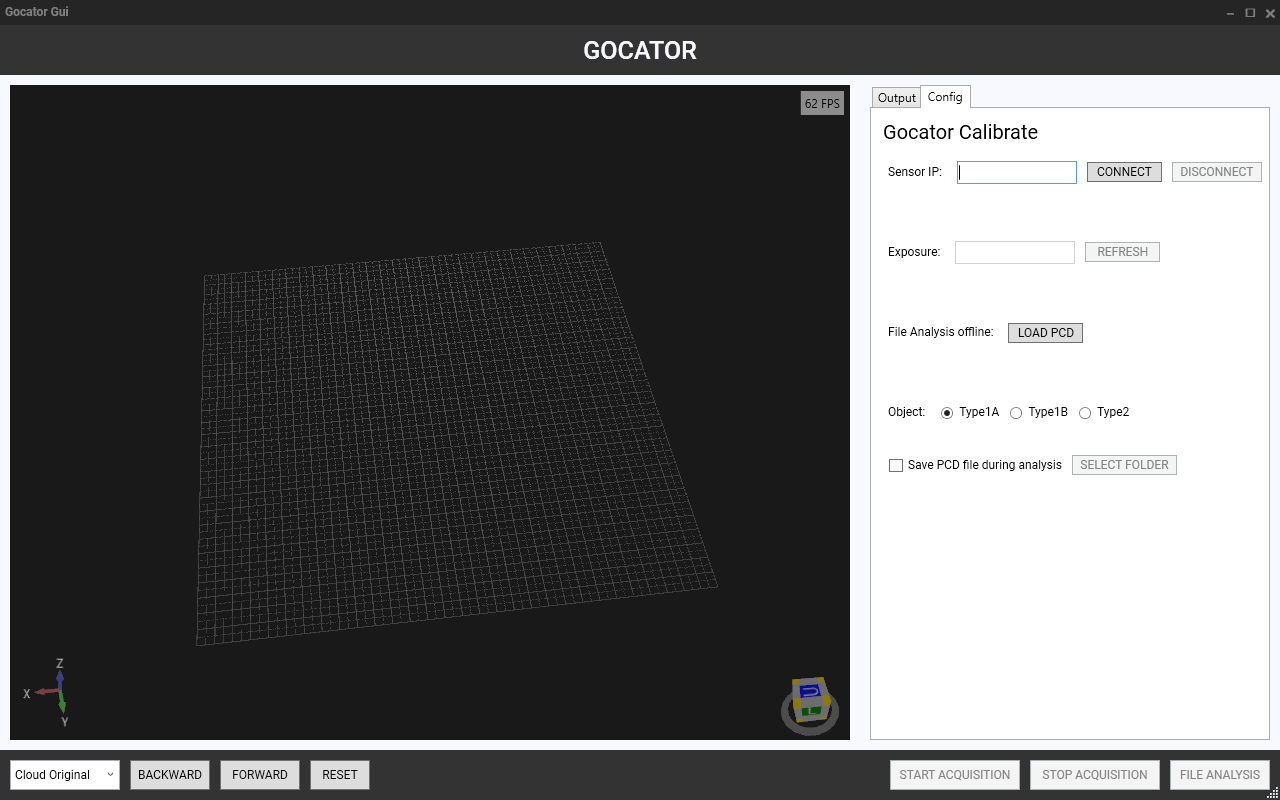
\includegraphics[width=0.9\columnwidth]{./pictures/gui_1.png}
	\caption{Interfaccia grafica del programma.}\label{fig:gui_1}
\end{figure}

\noindent Il programma può essere utilizzato sia in modalità online (connesso direttamente al Gocator) sia in modalità offline (caricando e analizzando il file della \textit{point cloud} del battistrada).\\
\newline
La modalità online permette di:

\begin{itemize}
	\item Inserire l'indirizzo IP del sensore, connettersi e disconnettersi;
	\item Modificare il valore dell'esposizione;
	\item Selezionare il tipo di battistrada da analizzare;
	\item Salvare i file in formato \textit{.pcd}, durante l'analisi, delle \textit{point cloud} step by step;
	\item Avviare e stoppare la scansione, con la visualizzazione del risultato dell'analisi in real time;
	\item Visualizzare a video le \textit{point cloud} dei battistrada scansionati e analizzati;
\end{itemize}

\noindent La modalità offline permette di:

\begin{itemize}
	\item Caricare un file contenente la \textit{point cloud} del battistrada;
	\item Selezionare il tipo di battistrada da analizzare;
	\item Salvare, durante l'analisi, le \textit{point cloud} step by step;
	\item Avviare l'analisi del file;
	\item Visualizzare a video le \textit{point cloud} caricate;
\end{itemize}

\begin{figure}[H]
	\centering
	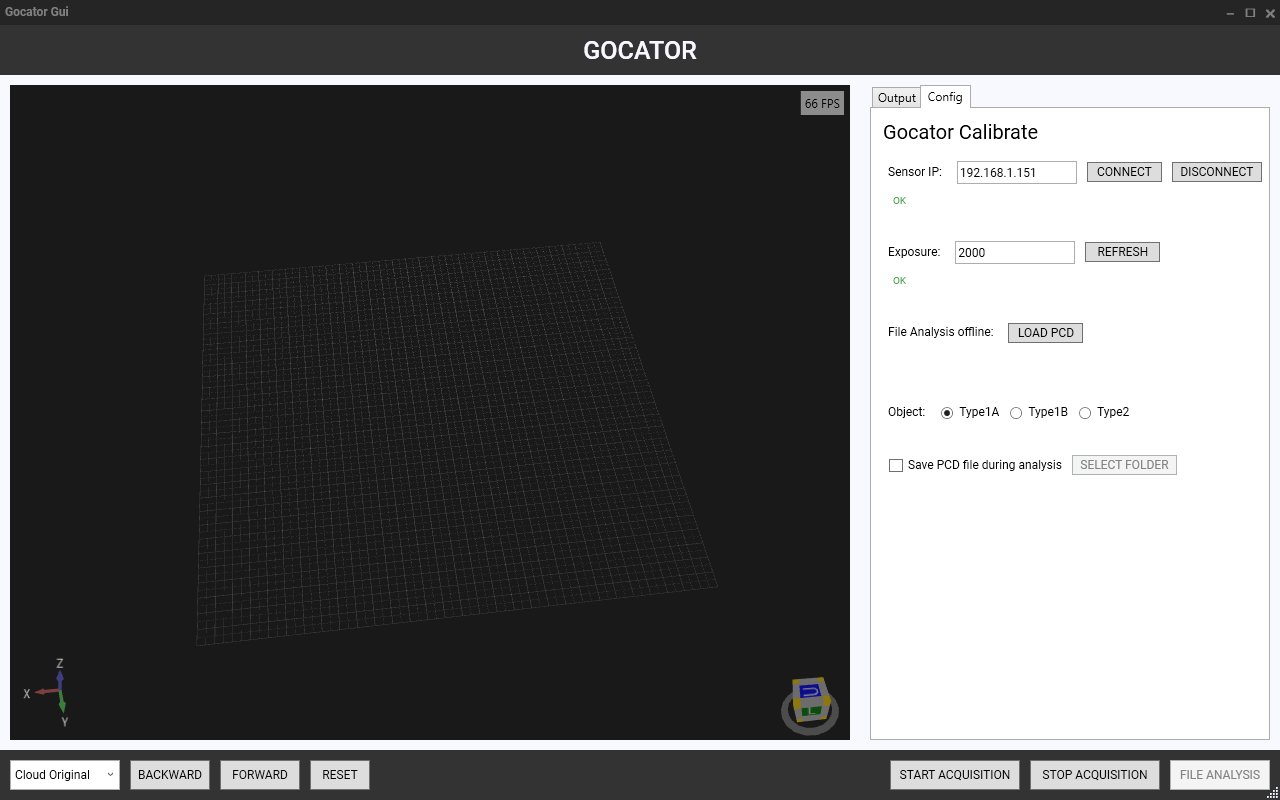
\includegraphics[width=0.9\columnwidth]{./pictures/gui_2.png}
	\caption{Interfaccia grafica con la point cloud filtrata visualizzata a video.}\label{fig:gui_2}
\end{figure}

\noindent In particolare, nel caso del battistrada di tipo \textit{2}, il risultato della scansione riporta a video, oltre alla \textit{point cloud} del battistrada, anche la stessa con evidenziati i punti di altezza delle scanalature minima e massima, e la \textit{point cloud} con solo i punti di massimo da sinistra e destra (figura \ref{fig:gui_4}, figura \ref{fig:gui_5} e figura \ref{fig:gui_6}).

\begin{figure}[H]
	\centering
	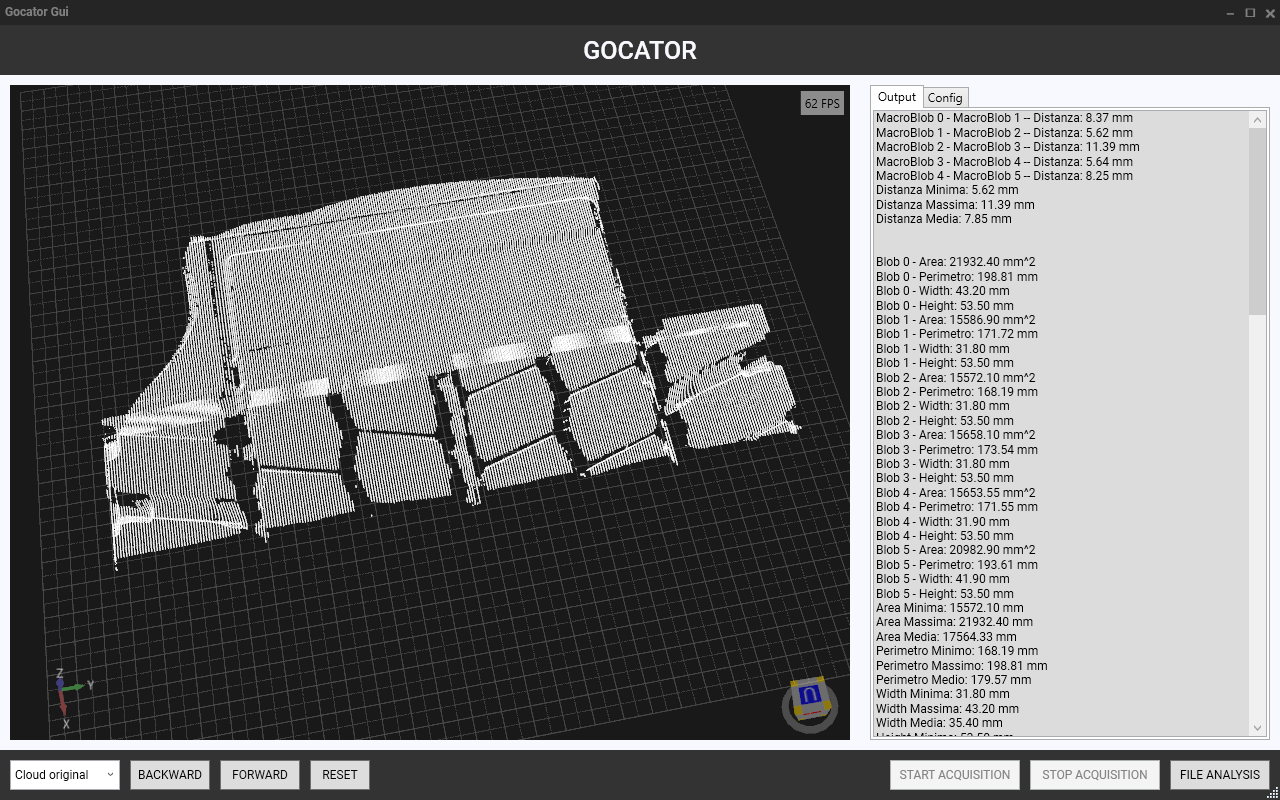
\includegraphics[width=0.9\columnwidth]{./pictures/gui_3.png}
	\caption{Interfaccia grafica con, visualizzata a video, la point cloud del battistrada di tipo 1A e il risultato dell'analisi.}\label{fig:gui_3}
\end{figure}

\begin{figure}[H]
	\centering
	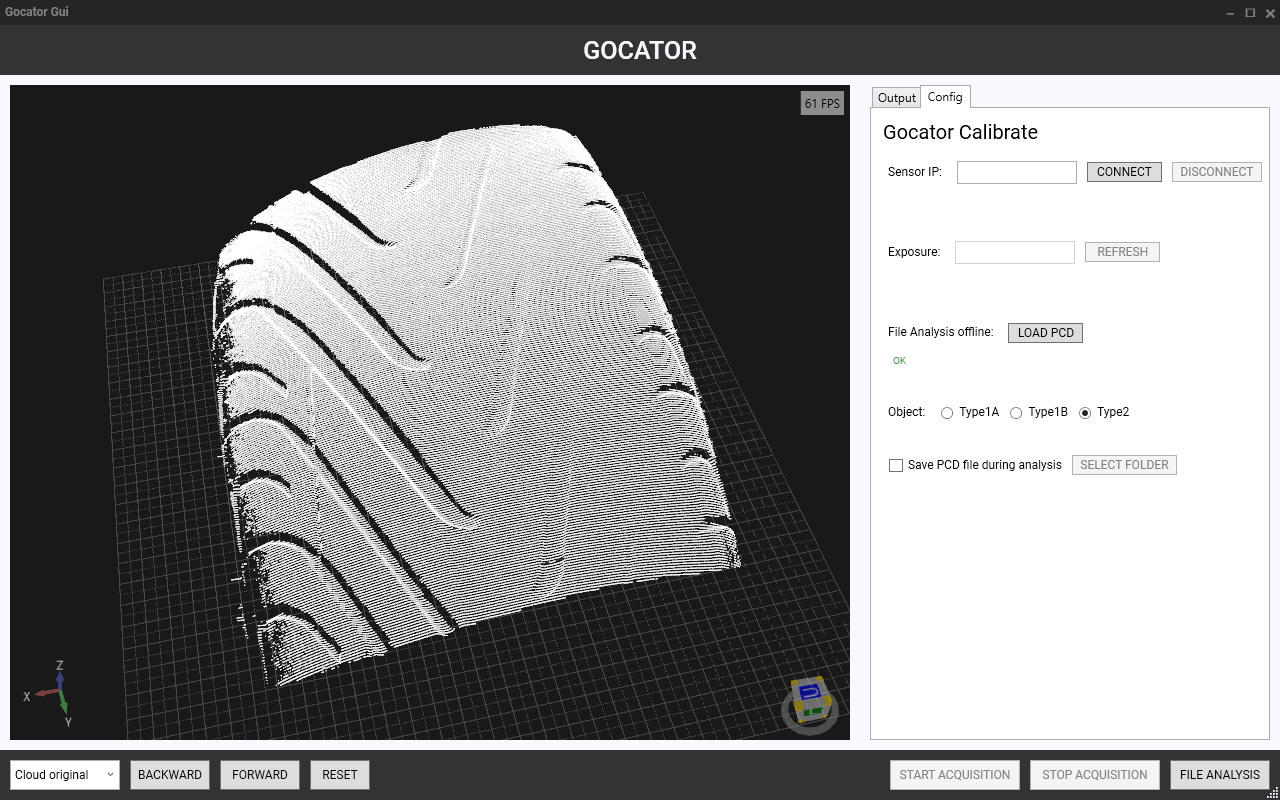
\includegraphics[width=0.9\columnwidth]{./pictures/gui_4.png}
	\caption{Interfaccia grafica con, visualizzata a video, la point cloud del battistrada di tipo 2.}\label{fig:gui_4}
\end{figure}

\begin{figure}[H]
	\centering
	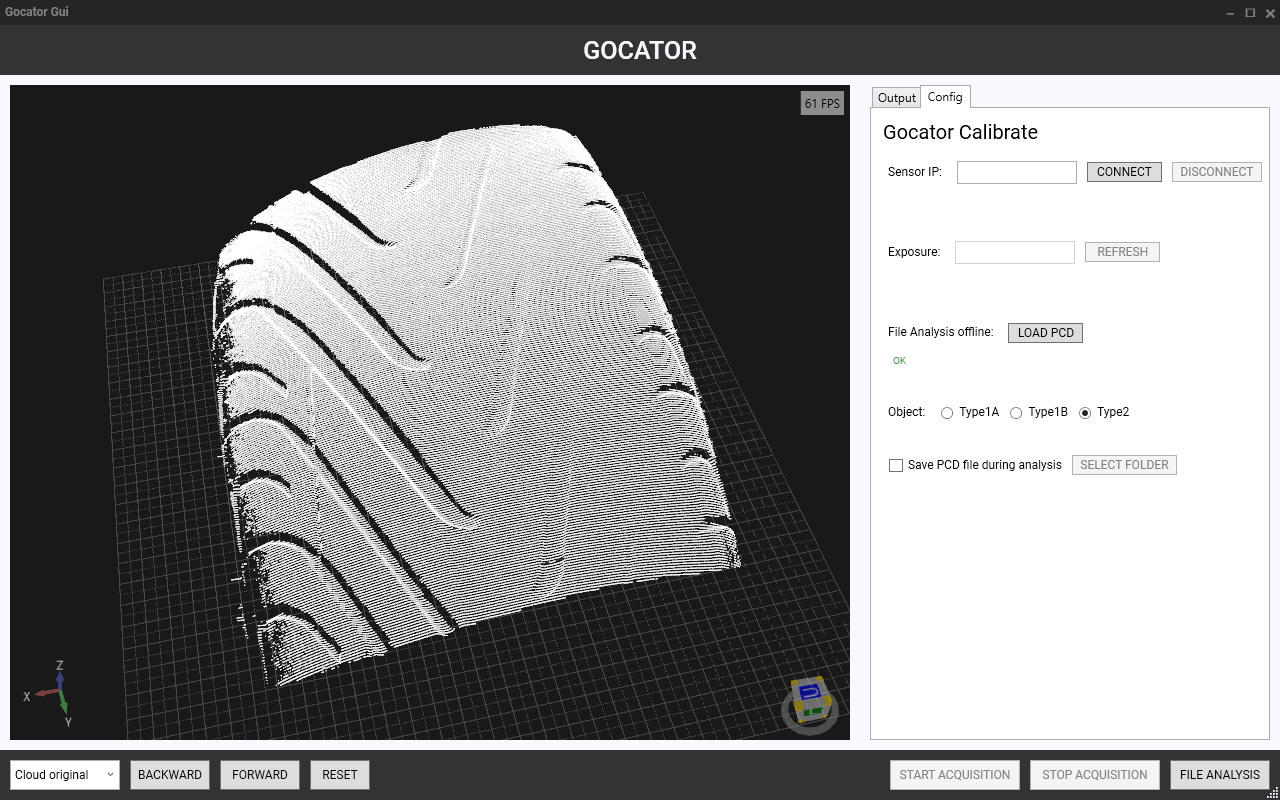
\includegraphics[width=0.9\columnwidth]{./pictures/gui_5.png}
	\caption{Interfaccia grafica con, visualizzata a video, la point cloud con i punti di profondità delle scanalature minima e massima.}\label{fig:gui_5}
\end{figure}

\begin{figure}[H]
	\centering
	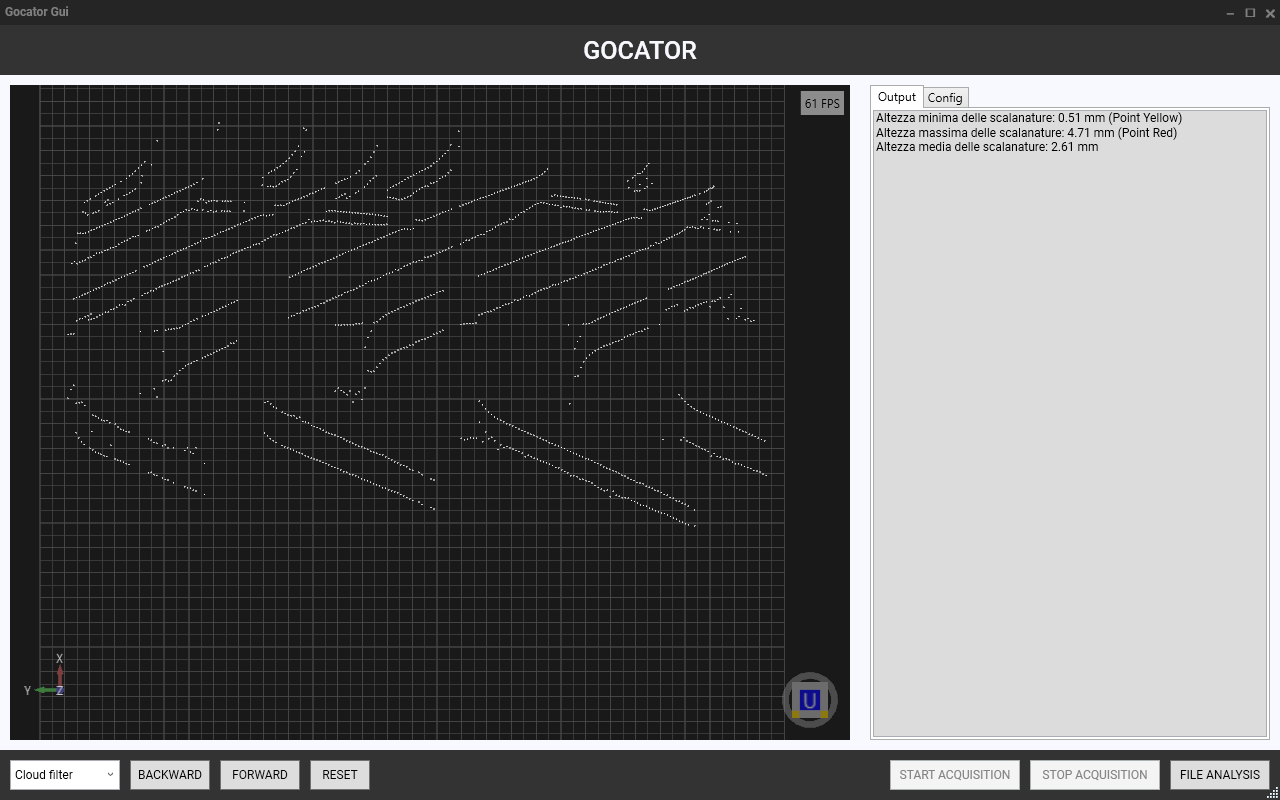
\includegraphics[width=0.9\columnwidth]{./pictures/gui_6.png}
	\caption{Interfaccia grafica con, visualizzata a video, la point cloud filtrata.}\label{fig:gui_6}
\end{figure}